\chapter{变分推断与确定性近似}
\label{chap:pgm-variational}

局部因子很小，联合推断仍可能很贵。第~\ref{chap:pgm-elimination}章和第~\ref{chap:pgm-junction-tree}章通过消元与团树保存了依赖关系；当中间团过大时，保存这些关系本身就成为瓶颈。此时可以改变问题：不再要求把后验完整算出来，而是在一个可计算的分布集合中寻找替代品。另一些任务只需要一组最可能的配置，则可以放宽配置必须满足的约束，先求一个较容易的优化问题。两条路线都把推断改写为优化，但前者近似的是概率分布，后者近似的是离散决策，不能用同一种“准确率”概括。

本章把模型参数视为已知。第一类查询以观测$\bm{x}$和潜变量$\bm{z}$的后验$p(\bm{z}\mid\bm{x})$为目标，输出合法近似分布、伪边缘或局部高斯近似，以便继续计算边缘概率和期望；第二类查询把证据吸收到因子中，输出全部未观测变量的一组联合最优配置，即最可能解释（most probable explanation, MPE）。选择怎样的近似对象、怎样衡量误差，以及怎样实际求解，是三个不同的决定。两类查询共享变分几何和局部计算工具，却不能用一类输出替代另一类答案。

图~\ref{fig:pgm-variational-query-map}从查询需求分流：需要边缘概率、期望或不确定性时，进入第~\ref{sec:pgm-variational-posterior}节；只需全部未观测变量的一组最大得分配置时，进入第~\ref{sec:pgm-variational-mpe}节。图中方法名是后文的阅读入口，不必预先掌握；同一分支内的近似族、计算组织与优化方式还可以组合。共同的优化表示在下一节建立。
\begin{figure*}[htbp]
  \centering
  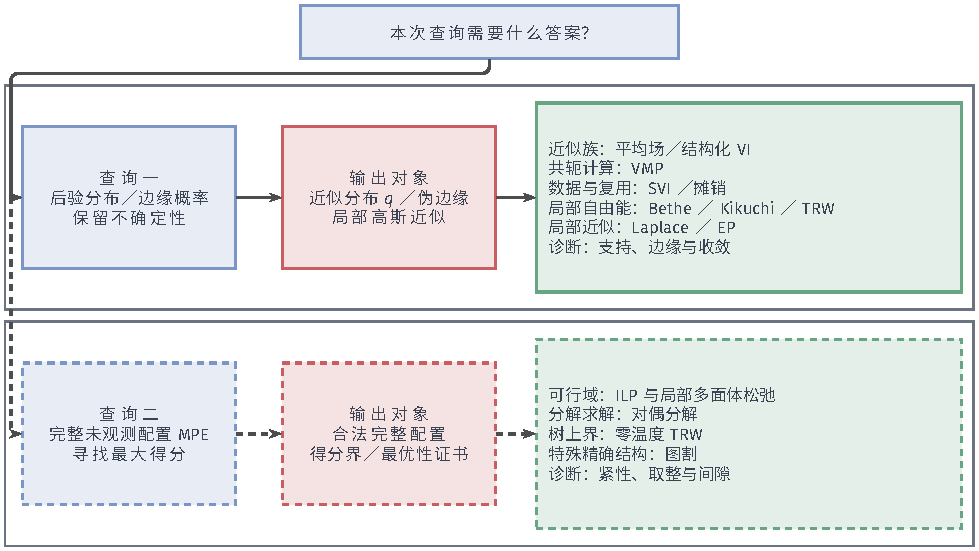
\includegraphics[width=\linewidth]{figures/03-models/03-probabilistic-graphical-models/tikz/pgm-variational-query-map/figure.pdf}
  \caption{按查询选择阅读路线。上支保留后验或边缘不确定性，下支回答完整配置MPE；图中的实线与虚线用于区分两支，不表示精确与近似。方法入口按所改变的对象分组，不是互斥算法清单。正温度TRW近似分布查询，零温度TRW提供MPE得分上界；含求和与最大化的边缘MAP不在本图范围内。}
  \label{fig:pgm-variational-query-map}
\end{figure*}
\FloatBarrier

\section{变分推断的统一视角}
\label{sec:pgm-variational-unified}
\label{sec:pgm-variational-duality}

设$p(\bm{x})$有限且为正；连续观测时，这里指观测位置的边缘密度。选取容易归一化、求期望或采样的分布族$\mathcal Q$，用$q\in\mathcal Q$代替难以直接计算的后验。\term{变分推断}（variational inference, VI）就是把寻找后验的任务变成选择分布的优化问题。它仍然输出不确定性，只是不再允许任意复杂的依赖关系。

目标直接沿用
\BookSectionRef{sec:information-elbo-approximation}{第一卷“数学准备”的目标分布逼近小节}。
令$\pi=p(\cdot\mid\bm x)$，要求$q\ll\pi$且$D_{\mathrm{KL}}(q\Vert\pi)<\infty$，
ELBO按整体对数比的期望定义：
\begin{equation}
  \begin{aligned}
    \mathcal L(q)
      &:=\mathbb E_q\log\frac{p(\bm x,\bm Z)}{q(\bm Z)},\\
    \log p(\bm{x})
      &=\mathcal L(q)+D_{\mathrm{KL}}(q\Vert\pi).
  \end{aligned}
  \label{eq:pgm-variational-elbo}
\end{equation}
整体期望不要求$\mathbb E_q\log p$和$\mathbb E_q\log q$分别有限；
后文把它写成$\mathbb E_q\log p+H(q)$时，另要求两项均有定义。
KL无限时可令ELBO为$-\infty$，但不能把$-\infty+\infty$当作合法分解。
模型固定时，最大化ELBO等价于最小化$D_{\mathrm{KL}}(q\Vert\pi)$；
这里的反向KL称谓只约定参数顺序。本节使用卷一的$D_{\mathrm{KL}}$记号，
本卷其他公式中的$\operatorname{KL}$是同一散度的简写。

式~\eqref{eq:pgm-variational-elbo}还分清了三类偏差。近似族过小，即使找到最优$q^\star$也无法表示后验，这是近似族限制。把反向KL换成正向KL、矩匹配或其他目标，改变的是“接近”的含义。实际算法停在$\widehat q$，还会留下$\mathcal L(q^\star)-\mathcal L(\widehat q)$的优化误差。若上确界没有达到，可用上确界代替$\mathcal L(q^\star)$。增加迭代只能尝试减少第三项，不能自动补回近似族已删去的依赖。

反向KL在$q$分配质量的位置评估误差。若$q$在$p=0$的区域放置正质量，KL会变成无穷大，因此近似分布必须避开目标不允许的位置。这是对目标零区域的回避；从$q$的角度，文献通常称其为\term{零强制}（zero forcing）：目标为零会迫使近似也为零。相对地，正向$\operatorname{KL}(p\Vert q)$的\term{零回避}（zero avoiding）要求$q$不能在$p$有正质量的位置为零。两种叫法关注的是$q$，不能仅凭“回避”二字判断KL方向\scite{bishop2006}

目标处处为正但存在低密度谷时，单峰$q$覆盖两个相隔很远的模态，可能需要把许多质量放进谷底；只覆盖一个模态则不必为另一个模态逐点支付损失。这解释了反向KL常见的模态选择倾向，却不是所有分布或所有近似族上的定理。足够丰富的混合分布族可以同时保留多个模态，单峰目标也未必产生模态遗漏。

一个可解析的例子能更准确地说明方差低估。设目标是零均值二维高斯，协方差为
\[
  \bm{\Sigma}=
  \begin{pmatrix}1&r\\r&1\end{pmatrix},
  \qquad |r|<1,
\]
并限制$q=\mathcal N(\bm{m},\operatorname{diag}(v_1,v_2))$。记精度矩阵$\bm{\Lambda}=\bm{\Sigma}^{-1}$，高斯KL的有关项为
\[
  \frac12\left\{\bm{m}^{\top}\bm{\Lambda}\bm{m}
     +\sum_i\bm{\Lambda}_{i,i}v_i-\sum_i\log v_i\right\}.
\]
对$\bm{m}$和$v_i>0$求导得到$\bm{m}=\bm{0}$、$v_i=1/\bm{\Lambda}_{i,i}=1-r^2$。取$r=0.8$时，目标的两个边缘方差均为$1$，最优独立近似却均为$0.36$。它选择的宽度接近给定另一坐标后的条件宽度，避免把质量放在狭长高斯等高线之外。相反，最小化$\operatorname{KL}(p\Vert q)$会匹配边缘矩，得到$v_i=1$。这个计算证明了当前高斯设定下的低估，不证明所有反向KL近似都低估所有方向的方差。

要把分布优化与图上的局部计算联系起来，使用
\BookSectionRef{sec:probability-common-distributions}{第一卷“数学准备”的指数族与分布模型小节}
建立的指数族形式。本节记自然参数为$\bm\theta$、统计量为$\bm T$，把可实现的统计量期望作为优化坐标：
\begin{equation}
  \begin{aligned}
    p_{\bm{\theta}}(\bm{z})
      &=h(\bm{z})\exp\{\langle\bm{\theta},\bm{T}(\bm{z})\rangle
                      -A(\bm{\theta})\},\\
    A(\bm{\theta})
      &=\log\int h(\bm{z})
          e^{\langle\bm{\theta},\bm{T}(\bm{z})\rangle}\,d\bm{z}.
  \end{aligned}
  \label{eq:pgm-variational-exponential-family}
\end{equation}
$h$为不依赖参数的基准项，$A$为对数配分函数。
自然参数位于$A<\infty$的开域内并满足微分积分交换条件时，沿用卷一的矩关系：
\begin{equation}
  \nabla A(\bm{\theta})=\mathbb E_{\bm{\theta}}\bm{T}(\bm{Z})
      =:\bm{\mu},\qquad
  \nabla^2 A(\bm{\theta})
      =\operatorname{Cov}_{\bm{\theta}}[\bm{T}(\bm{Z})].
  \label{eq:pgm-variational-moments}
\end{equation}
$\bm{\mu}$称为\term{均值参数}（mean parameter），直接记录期望统计量。
图模型常采用完整配置指示量，它们可能存在仿射冗余，因此即使$A$凸，也不能直接要求Hessian可逆。
只有在相应最小表示和内部条件下，才使用自然参数与均值参数的一一对应。

以下对偶与多面体陈述先限定为有限离散状态、$h=1$。以$V=\{1,\ldots,d\}$记节点集，$Z_i$的有限非空状态集为$\mathcal X_i$，节点集$A\subseteq V$上的配置集为$\mathcal X_A=\prod_{i\in A}\mathcal X_i$，全部联合配置组成$D=\mathcal X_V$。定义\term{边缘多面体}（marginal polytope）
\begin{equation}
  \mathcal M
    =\left\{\mathbb E_q\bm{T}(\bm{Z}):q\text{为全局分布}\right\}
    =\operatorname{conv}\{\bm{T}(\bm{z}):\bm{z}\in D\},
  \label{eq:pgm-variational-marginal-polytope}
\end{equation}
其中$\operatorname{conv}$表示凸包。当$\bm{T}$由节点和因子配置的指示函数组成时，$\bm{\mu}$就是相应边缘概率；$\mathcal M$要求这些局部表格能够同时来自某个全局分布，而不只是每张表各自归一化。

\BookTheoremRef{thm:information-finite-entropy-duality}{第一卷“数学准备”的有限配置最大熵对偶定理}
把配分函数改写为均值参数上的优化。对$\bm\mu\in\mathcal M$，
令$H^\star(\bm\mu)=\max_{q:\mathbb E_q\bm T=\bm\mu}H(q)$，则
\begin{equation}
  A(\bm\theta)=\max_{\bm\mu\in\mathcal M}
    \{\langle\bm\theta,\bm\mu\rangle+H^\star(\bm\mu)\}.
  \label{eq:pgm-variational-gibbs}
\end{equation}
该结论包含边界均值，不要求它由有限自然参数实现；
凸共轭在$\mathcal M$上为$-H^\star$，在外部为$+\infty$。
这里保留的是图推断要使用的目标与可行域，最大熵对偶的证明沿用卷一。

这里的负熵必须读成“给定统计量后的最大熵的负值”。少量边缘统计量通常不能确定任意全局分布，其熵不能随便代入$A^\star$。对一般基准项$h$，应把$H(q)$替换成$H(q)+\mathbb E_q\log h$；对连续变量，还需要可积性、闭性和对偶成立条件，均值可实现集合也通常不是有限多面体。指数族与变分对偶的系统处理见Wainwright和Jordan的专著式综述\scite{pgm-wainwright2008}

式~\eqref{eq:pgm-variational-gibbs}指出了两处困难：$\mathcal M$的全局一致性约束可能很多，$H^\star$也可能难算。平均场限制全局分布，保留真实熵，因此得到下界；局部自由能方法同时替换可行集合和熵，不再自动保留下界；配置优化去掉熵，再扩大可行集合，则得到最大得分的上界。这些方向来自具体的包含关系，不来自“变分”这个名称。

同一坐标也能表示MPE。令$S(\bm z)=\langle\bm{\theta},\bm T(\bm z)\rangle$为吸收证据后的有限离散得分，$D$为全部未观测变量的完整配置集合，则
\begin{equation}
  \max_{\bm z\in D}S(\bm z)
    =\max_{\bm{\mu}\in\mathcal M}
       \langle\bm{\theta},\bm{\mu}\rangle.
  \label{eq:pgm-variational-mpe}
\end{equation}
右侧没有熵项，因为答案只需保留一个最大得分配置，而无须累计其他配置的概率质量。对数配分函数查询若替换$\mathcal M$或$H^\star$，误差落在分布、边缘或归一化常数上；MPE若扩大$\mathcal M$，则得到连续松弛及最大得分上界，还必须从松弛解恢复合法配置。这正是两条主线共享几何表示而输出、保证和诊断不同的原因。

这个变分表示提供了比较方法的依据，却不意味着所有方法都在近似同一个自由能。第~\ref{sec:pgm-variational-laplace-ep}节的拉普拉斯近似改变众数附近的对数密度形状，EP匹配临时倾斜分布的矩；它们不直接求解式~\eqref{eq:pgm-variational-gibbs}中的优化。第~\ref{sec:pgm-variational-lp}节的LP则从无熵的式~\eqref{eq:pgm-variational-mpe}出发，只放宽配置的一致性约束。比较时需要分别问：改变的是密度、局部矩，还是可行集合？

\begin{example}[三角图的精确基准]
  \label{ex:pgm-variational-triangle}
  以下人工构造的二元模型贯穿本章。三个变量$Z_i\in\{0,1\}$组成三角图，每条边奖励端点取不同值：
  \begin{equation}
    p_\beta(\bm{z})=\frac{\exp S_\beta(\bm{z})}{Z_\beta},
    \qquad
    S_\beta(\bm{z})
      =\beta\sum_{(i,j)\in E}\mathbb I[z_i\ne z_j],
    \quad \beta=\log2.
    \label{eq:pgm-variational-triangle}
  \end{equation}
  两个全相同配置的得分为$0$，其余六个配置恰有两条不相等边，得分为$2\beta$。因此
  \[
    Z_\beta=2+6e^{2\beta}=26,\qquad
    p_\beta(Z_i=1)=\frac12,\qquad
    p_\beta(Z_i\ne Z_j)=\frac{8}{13}.
  \]
  每条边上，两个同值配置$(0,0)$与$(1,1)$各有概率$5/26$；两个异值配置$(0,1)$与$(1,0)$各有概率$4/13$。节点边缘都是均匀的，但节点并不独立；三个二元变量也不可能在每条边上都取不同值。
\end{example}

图~\ref{fig:pgm-variational-triangle}把同一模型的三种描述并列起来。删去依赖会丢失真实相关性，只检查每条边又可能接受根本不存在的联合配置。后面两类近似分别面对这两种风险。
\begin{figure}[htbp]
  \centering
  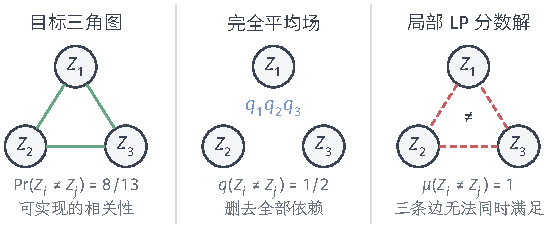
\includegraphics[width=\linewidth]{figures/03-models/03-probabilistic-graphical-models/tikz/pgm-variational-triangle/figure.pdf}
  \caption{三角图、完全因子化分布和局部一致的边缘表。右侧让每条边都以概率$1$取不同值，节点边缘仍都是$(1/2,1/2)$；它满足局部一致性，却不可能由任何全局二元分布实现。}
  \label{fig:pgm-variational-triangle}
\end{figure}

\section{近似后验分布与边缘概率}
\label{sec:pgm-variational-posterior}
\label{sec:pgm-variational-mean-field}

\subsection{从平均场到结构化变分}
\label{sec:pgm-variational-mean-field-structured}
\label{sec:pgm-variational-coordinate}

选择后验近似时，要把“保留哪些依赖”与“怎样算出近似”分开。平均场与结构化VI选择近似分布族；VMP组织共轭条件下的局部计算；SVI通过小批量减少一次全局更新需要处理的数据。它们不是四种互斥模型：选好近似族以后，还可以利用共轭消息和随机优化求解。后面的局部自由能、拉普拉斯近似与EP则进一步改变所维护的对象或匹配准则。

最直接的计算简化是让每个潜变量只保留自己的不确定性。\term{平均场近似}（mean-field approximation）采用
\[
  q(\bm{z})=\prod_{i=1}^{d}q_i(z_i).
\]
这一假设删去的是$q$中的后验依赖，不是原模型中的边。原模型的耦合仍通过期望进入更新；只是更新后的$q$无法表达“一个变量改变时，另一个变量的条件分布随之改变”。

固定除$q_i$之外的所有因子，记$q_{-i}=\prod_{j\ne i}q_j$，并定义$a_i(z_i)=\mathbb E_{q_{-i}}\log p(\bm{x},z_i,\bm{Z}_{-i})$。ELBO中依赖$q_i$的部分为
\[
  \int q_i(z_i)a_i(z_i)\,dz_i-\int q_i(z_i)\log q_i(z_i)\,dz_i.
\]
假设$C_i=\int e^{a_i(z_i)}dz_i$有限且为正，令$q_i^\star=e^{a_i}/C_i$，上述表达式就等于$\log C_i-\operatorname{KL}(q_i\Vert q_i^\star)$。KL在两分布相同时取唯一最小值，因此得到最优坐标更新：
\begin{equation}
  q_i^\star(z_i)
    \propto\exp\left\{\mathbb E_{q_{-i}}
      [\log p(\bm{x},z_i,\bm{Z}_{-i})]\right\}.
  \label{eq:pgm-variational-coordinate}
\end{equation}
期望只对其他变量计算，$z_i$在这一步是保留的自变量。更新使用的是对数联合分布的期望，再取指数；一般不等于$\mathbb E_{q_{-i}}p(z_i\mid\bm{x},\bm{Z}_{-i})$，也不等于把其他变量一律替换为其均值。

若原模型按因子分解，所有不含$z_i$的项都是归一化时可去掉的常数。平均场因此仍能局部更新。对例~\ref{ex:pgm-variational-triangle}，现在直接使用未归一化得分$S_\beta$，定义对数配分函数下界
\begin{equation}
  \begin{aligned}
    \mathcal L_Z(q)&=\mathbb E_qS_\beta(\bm Z)+H(q),\\
    \operatorname{KL}(q\Vert p_\beta)
      &=\log Z_\beta-\mathcal L_Z(q).
  \end{aligned}
  \label{eq:pgm-variational-partition-lower-bound}
\end{equation}
因此$\mathcal L_Z(q)\leq\log Z_\beta$。若使用已归一化的$p_\beta$计算$\mathbb E_q\log p_\beta+H(q)$，结果则是$\mathcal L_Z(q)-\log Z_\beta\leq0$，两者相差一个与$q$无关的常数。令$m_i=q_i(Z_i=1)$，并记$\mathcal L_{\mathrm{MF}}(\bm m)=\mathcal L_Z(\prod_iq_i)$，则
\begin{equation}
  \begin{aligned}
    \mathcal L_{\mathrm{MF}}(\bm m)
      &=\beta\sum_{(i,j)\in E}
           (m_i+m_j-2m_im_j)+\sum_i h_{\mathrm B}(m_i),\\
    m_i^{\mathrm{new}}
      &=\sigma\left(\beta\sum_{j\in N(i)}(1-2m_j)\right),
  \end{aligned}
  \label{eq:pgm-variational-triangle-mf}
\end{equation}
其中$\sigma(u)=1/(1+e^{-u})$，$h_{\mathrm B}(m)=-m\log m-(1-m)\log(1-m)$，$N(i)$是相邻节点集合。若两个邻居的$m_j$均为$1/4$，新$m_i=\sigma(\log2)=2/3$；邻居偏好$0$，当前变量便更偏好$1$。这不是硬性配置，而是伯努利分布参数。

均匀初始化给出固定点$m_i=1/2$，其对数配分函数下界为$\mathcal L_{\mathrm{MF}}=(9/2)\log2\approx3.119162$，低于$\log26\approx3.258097$。这一例中它还是平均场的全局最优：目标Hessian的对角元不大于$-4$，每行两个非对角元均为$-2\beta$，故最大特征值不超过$-4+4\beta<0$；目标在内部严格凹，熵导数又排除了边界最大点。然而$q(Z_i\ne Z_j)=1/2$，仍低于真实的$8/13$。全局解出了近似问题，并不等于消除了近似误差。

\begin{algorithm}[循环坐标平均场]
  \label{alg:pgm-variational-cavi}
  \begin{algorithmic}[1]
    \Require 联合分布、因子化近似族、有限ELBO的初值、容差$\varepsilon$
    \Ensure 近似分布$q$及其ELBO
    \State 计算当前ELBO
    \Repeat
      \State 保存本轮开始时的ELBO
      \For{$i=1,\ldots,d$}
        \State 用其他因子的最新值计算式~\eqref{eq:pgm-variational-coordinate}
        \State 归一化并替换$q_i$
      \EndFor
      \State 重新计算ELBO及本轮增量
    \Until{增量不超过$\varepsilon$，或达到计算预算}
  \end{algorithmic}
\end{algorithm}

算法~\ref{alg:pgm-variational-cavi}的每个精确坐标更新都不降低ELBO，因为它解出了当前坐标的最大化问题。由于ELBO有上界，目标值序列收敛。这个论证不保证参数序列收敛，也不保证一般模型中的全局最优；同时用旧值并行更新所有坐标也不受这个逐坐标证明保护。

平均场让坐标更新变得局部，却可能恰好拆开后验中最重要的依赖。例如，相邻隐状态高度相关时，逐点独立近似会把一条连贯轨迹变成许多互不协调的边缘。\term{结构化变分推断}（structured variational inference）在$q$中保留选定的依赖，用较贵的局部推断换取更强的表达能力。
\label{sec:pgm-variational-structured}

一种直接选择是把节点划分成互不相交的块$B_1,\ldots,B_K$，并让不同块独立，即
\[
  q(\bm z)=\prod_k q_k(\bm z_{B_k}).
\]
与单变量推导相同，固定其余块后，当前块的最优分布满足
\begin{equation}
  q_k^\star(\bm z_{B_k})
     \propto\exp\left\{
       \mathbb E_{q_{-B_k}}\log p(\bm x,\bm z_{B_k},\bm Z_{-B_k})
     \right\}.
  \label{eq:pgm-variational-block}
\end{equation}
块内部原有相互作用被保留，跨块作用转成期望势。链与小树都可以沿用第~\ref{sec:pgm-junction-tree-sum-product}节的和积消息；在链上向两个方向传递消息，就是后文时序模型使用的前向--后向计算。若是稠密大块，更新仍会遇到指数级枚举。因此，块大小只是粗略指标，块内树宽和因子的代数结构才决定计算代价。

回到三角图，取$q(z_1,z_2)q(z_3)$并令$q(z_3=1)=1/2$。两条跨块边的期望得分总和恒为$\beta$，所以
\[
  q(z_1,z_2)=
    \frac{e^{\beta\mathbb I[z_1\ne z_2]}}{2+2e^\beta}.
\]
当$\beta=\log2$时，块内不同值的概率为$2/3$，跨块边的不同值概率仍为$1/2$。该解也是块坐标固定点；它给出的对数配分函数下界为$\mathcal L_Z=\log(2+2e^\beta)+\beta+\log2=\log24\approx3.178054$，高于完全平均场的$3.119162$，但仍低于$\log26$。这里明确展示了增加结构保留了什么，也展示了两个尚未保留的相关性。

若$\mathcal Q_1\subseteq\mathcal Q_2$，对同一ELBO有$\sup_{\mathcal Q_1}\mathcal L\leq\sup_{\mathcal Q_2}\mathcal L$；这只是优化范围扩大的结果，不保证有限预算下求得的解也按此顺序改进。更一般的树结构$q$未必能分成互不相交的块，可以用树边缘及条件分布参数化，其熵仍能精确计算。无论采用哪种结构，只有$q$是合法全局分布、期望和真实熵计算正确时，ELBO下界才继续成立。结构化变分补回了选定依赖，却提高了每次坐标更新的成本；下一条路线固定近似族，转而利用共轭结构简化这些更新。

\subsection{从坐标更新到变分消息传递}
\label{sec:pgm-variational-coordinate-vmp}
\label{sec:pgm-variational-vmp}

式~\eqref{eq:pgm-variational-coordinate}虽然形式简洁，指数中的期望仍可能难算。若完整条件分布属于指数族，
\[
  \log p(z_i\mid\bm{z}_{-i},\bm{x})
    =\log h_i(z_i)
      +\langle\bm{\eta}_i(\bm{z}_{-i},\bm{x}),\bm T_i(z_i)\rangle
      +c(\bm{z}_{-i},\bm{x}),
\]
且相关期望存在，则更新后的$q_i$保持同一家族，自然参数为
\begin{equation}
  \bm{\lambda}_i
    =\mathbb E_{q_{-i}}\bm{\eta}_i(\bm{Z}_{-i},\bm{x}).
  \label{eq:pgm-variational-conjugacy}
\end{equation}
这就是条件共轭带来的计算闭合：期望改变参数，不改变函数形式。这里不要求$\bm{\eta}_i$对其他变量线性，但必须能够计算其期望，并确认结果落在合法自然参数域内。

在因子图中，设每个邻接因子的对数中与$z_i$有关的部分能写成$\langle\bm{\eta}_{a\to i}(\bm z_{S_a\setminus\{i\}}),\bm T_i(z_i)\rangle$。把$\log h_i$只计入一次，定义消息
\[
  \bm m_{a\to i}
    =\mathbb E_{q_{S_a\setminus\{i\}}}\bm{\eta}_{a\to i},
  \qquad
  \bm{\lambda}_i=\sum_{a:\,i\in S_a}\bm m_{a\to i}.
\]
变量再把$\mathbb E_{q_i}\bm T_i$发给邻接因子，以供后续期望计算。\term{变分消息传递}（variational message passing, VMP）就是这种以充分统计量和自然参数交换实现坐标优化的方式。消息不必是归一化概率表，也不同于和积算法对原因子先乘后求和的消息。它的基本闭式版本依赖所选因子化及条件共轭；非共轭模型需要局部界、数值积分或梯度更新，不能只写一句“传递消息”便认为期望已有解析解\scite{pgm-variational-winn2005}

例如，全局成功率$\Pi\sim\operatorname{Beta}(a_0,b_0)$，$Z_i\mid\Pi\sim\operatorname{Bernoulli}(\Pi)$，观测因子为$p(x_i\mid z_i)$。取$q(\pi)\prod_iq_i(z_i)$，记$r_i=q_i(Z_i=1)$，便有
\begin{equation}
  \begin{aligned}
    q(\pi)&=\operatorname{Beta}(a,b),\\
    a&=a_0+\sum_i r_i,\qquad
    b=b_0+\sum_i(1-r_i),\\
    \log\frac{r_i}{1-r_i}
      &=\mathbb E_q\log\Pi-\mathbb E_q\log(1-\Pi)
         +\log\frac{p(x_i\mid1)}{p(x_i\mid0)}.
  \end{aligned}
  \label{eq:pgm-variational-beta-bernoulli}
\end{equation}
其中$\mathbb E\log\Pi=\psi(a)-\psi(a+b)$、$\mathbb E\log(1-\Pi)=\psi(b)-\psi(a+b)$，$\psi(u)=d\log\Gamma(u)/du$是双伽马函数。局部变量向全局因子发送的是软计数$(r_i,1-r_i)$，全局变量返回的是期望对数概率，而不是$\log\mathbb E\Pi$。

取$a_0=b_0=1$，两个样本的似然比分别为$4$和$1/4$。从$q(\pi)=\operatorname{Beta}(1,1)$开始，局部更新给出$r_1=0.8,r_2=0.2$；全局更新得到$\operatorname{Beta}(2,2)$。由于新的两个期望对数概率仍相等，再次局部更新不变。计算过程只传递两个软计数及两个期望，不枚举$(Z_1,Z_2,\Pi)$的联合状态；代价是$q$不再保留$\Pi$与$Z_i$之间的后验相关。

\subsection{从批量优化到随机与摊销推断}
\label{sec:pgm-variational-stochastic-amortized}
\label{sec:pgm-variational-scalable}
\label{sec:pgm-variational-svi}

即使每个局部更新便宜，遍历全部$n$个样本才能改变一次全局参数，也会拖慢大数据推断。设全局潜变量为$\bm u$，样本局部潜变量为$\bm z_i$，
\[
  p(\bm u,\bm z_{1:n},\bm x_{1:n})
    =p(\bm u)\prod_{i=1}^n p(\bm x_i,\bm z_i\mid\bm u),
  \qquad
  q=q_{\bm{\lambda}}(\bm u)\prod_iq_{\bm{\phi}_i}(\bm z_i).
\]
假设共轭使全局完整条件分布的自然参数等于$\bm{\lambda}_0+\sum_i\bm s(\bm x_i,\bm z_i)$。固定局部因子时，最优全局自然参数为$\bm{\lambda}^\star=\bm{\lambda}_0+\sum_i\mathbb E_{q_i}\bm s_i$。

普通欧氏梯度没有考虑不同参数方向会引起多大的分布变化。\term{自然梯度}（natural gradient）用Fisher信息矩阵校正梯度，使更新按分布的局部几何衡量。在最小、正则指数族内部，记全局对数配分函数为$A_q$，则$\bm F(\bm{\lambda})=\nabla^2 A_q(\bm{\lambda})$。全局ELBO中依赖$\bm{\lambda}$的部分为
\[
  \langle\bm{\lambda}^\star-\bm{\lambda},
            \nabla A_q(\bm{\lambda})\rangle+A_q(\bm{\lambda})+C.
\]
求导得到$\nabla_{\bm{\lambda}}\mathcal L=\bm F(\bm{\lambda})(\bm{\lambda}^\star-\bm{\lambda})$，从而
\begin{equation}
  \widetilde\nabla_{\bm{\lambda}}\mathcal L
    =\bm{\lambda}_0+\sum_i\mathbb E_{q_i}\bm s_i-\bm{\lambda}.
  \label{eq:pgm-variational-natural-gradient}
\end{equation}
若局部因子已经达到给定全局参数下的最优值，在可微等条件下，包络定理允许用这同一偏导计算优化掉局部变量后的目标梯度。

均匀抽取大小为$b$的小批量$B$，更新其中局部因子后，用
\begin{equation}
  \begin{aligned}
    \widehat{\bm{\lambda}}
      &=\bm{\lambda}_0+\frac{n}{b}
           \sum_{i\in B}\mathbb E_{q_i}\bm s_i,\\
    \bm{\lambda}^{(t+1)}
      &=(1-\rho_t)\bm{\lambda}^{(t)}
          +\rho_t\widehat{\bm{\lambda}}
  \end{aligned}
  \label{eq:pgm-variational-svi}
\end{equation}
即可得到\term{随机变分推断}（stochastic variational inference, SVI）。在给定当前全局参数并精确求解相应局部问题时，缩放的统计量和是全数据和的无偏估计。非均匀抽样需要按纳入概率加权；局部更新不充分则还会引入偏差，不能仅凭随机抽样宣称梯度无偏\scite{pgm-variational-hoffman2013}

在式~\eqref{eq:pgm-variational-beta-bernoulli}中，若$n=1000$，抽到的$10$个样本的$r_i$之和为$7$，先验仍为$\operatorname{Beta}(1,1)$，则小批量给出的目标分布是$\operatorname{Beta}(701,301)$。若当前分布为$\operatorname{Beta}(501,501)$，取步长$0.1$，更新为$\operatorname{Beta}(521,481)$。缩放发生在统计量而不是先验上，否则会把先验重复计算。

常见递减步长满足$\sum_t\rho_t=\infty$、$\sum_t\rho_t^2<\infty$，如$\rho_t=(t+t_0)^{-\kappa}$、$1/2<\kappa\leq1$。结合光滑性、迭代有界、噪声矩受控等随机逼近条件，可以得到趋向驻点的结论；这两个步长条件单独并不是完整收敛定理。每一步的ELBO也不必上升。局部更新负责解释当前样本，全局更新负责汇总统计量，两者的分工决定了小批量并行与内存节约。

至此可以按实际瓶颈选择组合。若主要关心单变量边缘、内存紧张，完全平均场可作为成本较低的起点，但仍需检查遗漏相关性是否影响所需统计量；若需要相邻状态的联合概率或整段轨迹，应考虑保留链或小块依赖，并承担块内推断成本。增加结构是否值得，要看这些依赖是否影响当前查询，而不只看ELBO是否提高。

近似族选定后，条件共轭且统计量期望可算时，可用VMP组织更新；它本身不补回被因子化删除的相关性。若瓶颈是遍历大量样本，且模型具有上述可分解的局部统计量和全局更新，则可叠加SVI，用有噪声的小批量更新换取较低的单步成本。例如每个样本是一段序列时，可以在局部因子$q_{\bm\phi_i}(\bm z_i)$中保留整条链，精确计算链内统计量，再用小批量更新共轭的全局参数。这样同时用了结构化近似、可解析的消息计算和SVI；小批量并不会降低一条链内部的推断复杂度。

\label{sec:pgm-variational-amortized}

小批量减少了每次读取的数据，却仍需为每个新样本求解局部优化。若样本不断到来，可以学习一个共享映射$\bm{\phi}_i=f_{\bm{\omega}}(\bm x_i)$，直接输出$q_{\bm{\phi}_i}(\bm z_i)$的参数。\term{摊销推断}（amortized inference）把许多样本的推断计算转移到一次共享训练中；测试时主要执行前向计算，也可以在其输出上继续作样本级优化。

非共轭模型下，ELBO的期望通常用采样估计。对于能够写成$\bm z=g_{\bm{\phi}}(\bm\epsilon)$、$\bm\epsilon\sim r(\bm\epsilon)$且$r$不依赖$\bm{\phi}$的分布，随机性可以与参数分开。例如高斯分布可写为$\bm z=\bm m+\bm L\bm\epsilon$，$\bm\epsilon\sim\mathcal N(\bm0,\bm I)$，$\bm L\bm L^\top$为协方差。令$F_{\bm{\phi}}(\bm z)=\log p(\bm x,\bm z)-\log q_{\bm{\phi}}(\bm z)$，在可交换微分与期望的可积支配条件下，
\begin{equation}
  \begin{aligned}
    \nabla_{\bm{\phi}}\mathcal L
      =\mathbb E_r\big[
        &(\nabla_{\bm{\phi}}g_{\bm{\phi}})^\top
           \nabla_{\bm z}F_{\bm{\phi}}
                (g_{\bm{\phi}}(\bm\epsilon))\\
        &+\left.\nabla_{\bm{\phi}}F_{\bm{\phi}}(\bm z)
          \right|_{\bm z=g_{\bm{\phi}}(\bm\epsilon)}
        \big].
  \end{aligned}
  \label{eq:pgm-variational-pathwise}
\end{equation}
第二行对$\bm z$保持固定，只微分$F$的显式参数依赖；第一行则跟踪样本位置随参数移动的影响。这是\term{重参数化梯度}（reparameterization gradient），也称路径导数估计：先把期望写到固定噪声上，再用链式法则求导。它不是把采样算子直接当成常数。模型也含待学习参数时，应另加对应的显式偏导。一般推导可用于多种潜变量模型，第~\ref{chap:pgm-generative}章将在VAE中实例化，不再重复这一计算\scite{kingma2013}

以$q=\mathcal N(m,s^2)$、$s>0$和$f(z)=z^2$为例，$z=m+s\epsilon$，路径导数的单样本估计分别是$2(m+s\epsilon)$与$2(m+s\epsilon)\epsilon$，期望为$2m$与$2s$，恰与$\partial_m(m^2+s^2)$、$\partial_s(m^2+s^2)$一致。有限样本估计仍有方差，“可重参数化”不表示梯度无噪声，也不无条件保证它比其他估计器方差小。

离散变量的普通采样映射对参数通常是阶梯函数，几乎处处导数为零，直接套用路径导数不能得到正确梯度。若支持集固定，可改用
\begin{equation}
  \nabla_{\bm{\phi}}\mathbb E_{q_{\bm{\phi}}}f_{\bm{\phi}}(\bm Z)
    =\mathbb E_q\!\left[
       f_{\bm{\phi}}(\bm Z)\nabla_{\bm{\phi}}\log q_{\bm{\phi}}(\bm Z)
       +\nabla_{\bm{\phi}}f_{\bm{\phi}}(\bm Z)\right].
  \label{eq:pgm-variational-score-function}
\end{equation}
这称为\term{分数函数估计}（score-function estimator），其中“分数”指对数密度对参数的导数。它从$\nabla q=q\nabla\log q$直接得到。减去不依赖所采变量的基线不改变第一项期望，因为$\mathbb E_q\nabla\log q=0$，却可能降低方差。小状态空间也可以精确求和；连续松弛则用可微随机变量替代离散变量，一般改变了目标或引入偏差。支持集随参数变化时，还必须处理积分边界，不能照搬固定支持的等式。

摊销带来的速度收益应与误差分开衡量。为给出逐样本分解，以下改用固定生成参数$\bm\theta$、样本间相互独立的局部潜变量模型，并定义局部ELBO：
\[
  \begin{aligned}
    p_{\bm\theta}(\bm x_{1:n},\bm z_{1:n})
      &=\prod_i p_{\bm\theta}(\bm x_i,\bm z_i),\\
    \mathcal L_i(\bm\phi)
      &=\mathbb E_{q_{\bm\phi}}
          \log p_{\bm\theta}(\bm x_i,\bm Z_i)+H(q_{\bm\phi}).
  \end{aligned}
\]
这不同于前面的SVI层次模型：共享随机量$\bm u$被积分掉以后，各样本一般不独立，不能把联合对数证据拆成逐样本对数证据之和；其ELBO还包含全局因子的贡献。

在上述独立模型中，令$\mathcal L_i^\star=\sup_{\bm{\phi}}\mathcal L_i(\bm{\phi})$；设共享网络达到其最优参数$\bm{\omega}^\star$，实际训练结果为$\widehat{\bm{\omega}}$。假设以下各目标值有限，对同一批样本有
\begin{equation}
  \begin{aligned}
    &\sum_i\log p_{\bm\theta}(\bm x_i)
       -\sum_i\mathcal L_i(f_{\widehat{\bm{\omega}}}(\bm x_i))\\
    ={}&\sum_i[\log p_{\bm\theta}(\bm x_i)-\mathcal L_i^\star]\\
     &+\left[\sum_i\mathcal L_i^\star
          -\sum_i\mathcal L_i(f_{\bm{\omega}^\star}(\bm x_i))\right]\\
     &+\left[\sum_i\mathcal L_i(f_{\bm{\omega}^\star}(\bm x_i))
          -\sum_i\mathcal L_i(f_{\widehat{\bm{\omega}}}(\bm x_i))\right].
  \end{aligned}
  \label{eq:pgm-variational-amortization-gap}
\end{equation}
三项分别是近似族误差、共享映射限制带来的摊销误差和网络优化误差，按定义均非负。若最优值未取得，改用上确界解释。总体和的非负性不保证每个样本上的网络最优解都优于实际解；训练还必须在同一固定模型下比较。关于近似与摊销两类误差的区分，可参见Cremer等人的分析\scite{pgm-variational-cremer2018}

这些误差描述的是对模型后验的逼近。若生成模型本身遗漏了现实中的因素，即使后验推断精确，预测也可能失准；这种模型失配不能从式~\eqref{eq:pgm-variational-amortization-gap}直接读出。共享训练同时调整生成模型时，后验与近似族还会相互适应，因此不能把训练ELBO的全部改善都归因于推断更准确。

\subsection{从Bethe到Kikuchi局部自由能}
\label{sec:pgm-variational-bethe-kikuchi}
\label{sec:pgm-variational-local-free-energy}
\label{sec:pgm-variational-bethe}

结构化平均场把部分依赖保存在一个合法$q$中。另一种思路是不先构造全局$q$，而是直接维护节点和因子的局部概率表。以下设有限离散因子图的目标为$p(\bm z)=Z^{-1}\prod_a\psi_a(\bm z_{S_a})$，所有因子严格正，每个变量至少邻接一个因子。观测已吸收到$\psi_a$中。令$N(i)$为变量$i$的邻接因子集合，$d_i=|N(i)|$。树上的和积消息是
\begin{equation}
  \begin{aligned}
    n_{i\to a}(z_i)
      &\propto\prod_{b\in N(i)\setminus\{a\}}m_{b\to i}(z_i),\\
    m_{a\to i}(z_i)
      &\propto\sum_{\bm z_{S_a\setminus\{i\}}}
            \psi_a(\bm z_{S_a})
            \prod_{j\in S_a\setminus\{i\}}n_{j\to a}(z_j).
  \end{aligned}
  \label{eq:pgm-variational-lbp}
\end{equation}
树上去掉一条边会分离两个子图，因此消息汇总的是互不重复的变量集合；完整的双向传递可得精确边缘。在含环图上照用同一更新，就是\term{环置信传播}（loopy belief propagation, LBP）。环使传回的信息可能已经受过当前节点的影响，树上的独立分支解释随之失效。

算法从消息读出
\[
  b_i(z_i)\propto\prod_{a\in N(i)}m_{a\to i}(z_i),
  \qquad
  b_a(\bm z_{S_a})\propto\psi_a(\bm z_{S_a})
                         \prod_{i\in S_a}n_{i\to a}(z_i).
\]
这些$b_i,b_a$称为\term{伪边缘}（pseudomarginal）：它们被当成边缘概率使用，但暂未保证存在一个共同的全局分布。将非负、归一化及
\begin{equation}
  \sum_{\bm z_{S_a\setminus\{i\}}}b_a(\bm z_{S_a})=b_i(z_i),
  \qquad i\in S_a
  \label{eq:pgm-variational-local-consistency}
\end{equation}
组成的约束集合记为$\mathcal L$，称为\term{局部多面体}（local polytope）。它只检查因子与节点是否一致，故$\mathcal M\subseteq\mathcal L$；在含环图上包含关系可能严格。

局部表格如何组成熵？每个因子熵已经包含其中节点的熵，直接相加会重复计数。树结构恰好允许减掉多算的部分：
\begin{equation}
  \begin{aligned}
    H_{\mathrm B}(\bm b)
      &=\sum_aH(b_a)+\sum_i(1-d_i)H(b_i),\\
    F_{\mathrm B}(\bm b)
      &:=-\sum_a\mathbb E_{b_a}\log\psi_a-H_{\mathrm B}(\bm b).
  \end{aligned}
  \label{eq:pgm-variational-bethe}
\end{equation}
$F_{\mathrm B}$是\term{Bethe自由能}（Bethe free energy），即负的期望对数得分再减去局部熵近似。最小化自由能等价于最大化相应的得分加熵，但一般不等价于最大化某个合法$q$的ELBO。

树上为何可以精确使用这个熵公式？对正的局部一致$\bm b$，构造
\[
  q_{\mathrm T}(\bm z)=
    \frac{\prod_a b_a(\bm z_{S_a})}
         {\prod_i b_i(z_i)^{d_i-1}}.
\]
从叶端向内求和时，每次用局部一致性消去一个分支，最终得到$1$；保留任一节点或因子而消去其余分支，就得到对应的$b_i$或$b_a$。对$\log q_{\mathrm T}$求期望给出$H(q_{\mathrm T})=H_{\mathrm B}(\bm b)$。任何具有相同局部边缘的分布$q$都满足$\mathbb E_q\log q_{\mathrm T}=\mathbb E_{q_{\mathrm T}}\log q_{\mathrm T}$，于是$\operatorname{KL}(q\Vert q_{\mathrm T})=H_{\mathrm B}(\bm b)-H(q)\geq0$。因此$H_{\mathrm B}$正是这些边缘下的最大熵，$\mathcal L=\mathcal M$，式~\eqref{eq:pgm-variational-gibbs}适用。含零边缘的树情形可由条件分布构造或取极限处理；含环图则不能重复这段消叶证明。

\begin{theorem}[正消息固定点与Bethe驻点]
  \label{thm:pgm-variational-bp-stationary}
  设有限因子图中的每个变量具有有限非空状态空间且至少邻接一个因子，每个因子$\psi_a$均取有限严格正值。令$\mathcal L$为由非负性、归一化及式~\eqref{eq:pgm-variational-local-consistency}定义的局部多面体，$F_{\mathrm B}$为式~\eqref{eq:pgm-variational-bethe}定义的Bethe自由能。按任一固定正归一化约定，LBP正消息固定点所产生的伪边缘是$F_{\mathrm B}$在$\mathcal L$相对内部的驻点。反之，$\mathcal L$中的每个正内部驻点都能由一组满足式~\eqref{eq:pgm-variational-lbp}的正消息表示，消息的正比例缩放不影响伪边缘。
\end{theorem}
\begin{proof}
  为约束$\sum_{\bm z_{S_a\setminus\{i\}}}b_a-b_i=0$引入乘子$\lambda_{a,i}(z_i)$，另加归一化乘子。对$b_a$的驻点条件给出
  \[
    b_a\propto\psi_a\prod_{i\in S_a}n_{i\to a},
    \qquad n_{i\to a}=e^{-\lambda_{a,i}}.
  \]
  对$b_i$的驻点条件为$(1-d_i)\log b_i-\sum_a\lambda_{a,i}=\text{常数}$，即$\prod_a n_{i\to a}\propto b_i^{d_i-1}$。定义$m_{a\to i}$为式~\eqref{eq:pgm-variational-lbp}第二行的求和。局部一致性给出$b_i\propto n_{i\to a}m_{a\to i}$。把它对$a\in N(i)$相乘并使用前一乘积关系，得到$b_i\propto\prod_a m_{a\to i}$，继而得到第一行消息方程。这一推导没有除以$d_i-1$，因此也覆盖叶节点。

  反过来，固定点消息满足这两组乘积关系，且由消息更新保证局部一致性。取$\lambda_{a,i}=-\log n_{i\to a}$，剩余与状态无关的常数由归一化乘子吸收，即满足上述全部驻点条件。
\end{proof}

驻点可以是局部极小点、鞍点或退化点，定理没有把迭代变成下降算法。一般含环图的Bethe熵不保证凹；LBP可能振荡，也可能随初值到达不同固定点。阻尼更新$\log m^{\mathrm{new}}\leftarrow(1-\gamma)\log m^{\mathrm{old}}+\gamma\log\widetilde m$再归一化，常用于减轻振荡，但不构成普遍收敛保证。严格正性及内部条件也不能省略：硬约束引入零概率后，需要另外处理边界和不可定义的消息比值。固定点与自由能关系的原始论证见Yedidia等人\scite{pgm-variational-yedidia2005}

三角图提供了一个收敛却不精确的例子。均匀消息本身就是固定点，给出$b_i=(1/2,1/2)$、$b_{i,j}(0,1)=b_{i,j}(1,0)=1/3$、$b_{i,j}(0,0)=b_{i,j}(1,1)=1/6$。边上不同值的概率$2/3$不同于真实的$8/13$。代入式~\eqref{eq:pgm-variational-bethe}得到$-F_{\mathrm B}=3\log3=\log27>\log26$，所以它不是对数配分函数下界。

这个例子还能检验界方向。暂把$\beta$改为任意实数，令$r=e^\beta>0$，同一均匀固定点给出$Z_{\mathrm B}=(1+r)^3$，精确值是$Z=2+6r^2$，二者相差$(r-1)^3$。当$r=2$时Bethe高估，当$r=1/2$时$Z_{\mathrm B}=27/8<7/2=Z$，则低估。节点边缘在两种情况下都仍然精确；局部边缘、配分函数和联合依赖的误差不能混为一谈。

\label{sec:pgm-variational-kikuchi}

Bethe近似把树上的精确熵分解延伸到含环图，只需节点和原因子作用域上的伪边缘，代价是短环约束可能丢失。三角图的问题不能靠更精确地归一化一条边解决，因为缺失的是三条边共同闭合时的约束。Kikuchi近似改变的是区域大小和重复计数方式：直接维护覆盖一个短环的联合表格，再协调重叠区域的边缘。\term{区域}（region）在这里包含一组变量及分配给它的模型因子；区域越大，能同时检查的依赖就越多。

一种标准构造从覆盖全部原因子的最大区域出发，加入所需非空交集，形成按包含关系连接的有向无环区域图。用$R$表示区域的变量集合，$b_R$是其归一化伪边缘。对父区域$R$及子区域$S\subset R$要求$\sum_{\bm z_{R\setminus S}}b_R=b_S$。每个区域的\term{计数数}（counting number）$c_R$纠正重叠造成的重复计数；对按包含关系闭合的构造，可递归设
\begin{equation}
  c_R=1-\sum_{R'\supsetneq R}c_{R'}.
  \label{eq:pgm-variational-counting}
\end{equation}
需要检查每个原变量和每个原因子在包含它的区域中的计数总和均为$1$，并保证涉及同一变量或因子的区域通过相应包含边连通。任意选几块区域再任意给权重，并不能自动获得合法的区域近似。

令$\Theta_R(\bm z_R)=\sum_{a:S_a\subseteq R}\log\psi_a(\bm z_{S_a})$，并假设上述因子计数条件成立，则
\begin{equation}
  \begin{aligned}
    H_{\mathrm K}(\bm b)&=\sum_R c_R H(b_R),\\
    F_{\mathrm K}(\bm b)
      &=\sum_R c_R\left[
          \sum_{\bm z_R}b_R(\bm z_R)\log b_R(\bm z_R)
          -\mathbb E_{b_R}\Theta_R\right].
  \end{aligned}
  \label{eq:pgm-variational-kikuchi}
\end{equation}
这是\term{Kikuchi自由能}（Kikuchi free energy）的一种区域表示。因子计数和区域一致性使能量项仍把每个原因子计算一次，近似发生在熵及全局一致性上。若不同因子作用域至多共享一个变量，Bethe对应只用因子区域和单节点区域的特殊选择。一般因子图的Bethe仍属于区域自由能，但当因子共享多个变量时，未必等同于上述按全部交集闭合的Kikuchi构造。Kikuchi可以覆盖短环并约束更大的联合表格，不是把同一组单节点消息换个名字。

例如，在$3\times3$节点网格中选择四个小方格为最大区域，如图~\ref{fig:pgm-variational-regions}。四个方格各计$+1$；两方格共享的四条内部边各计$-1$；中央节点被四个方格及四条内部边共同覆盖，故还需计$1-4+4=+1$。边界交集的计数为$0$，可以保留作一致性约束，也可在不改变约束含义时省去。相应熵为“四个方格熵之和，减四条内部边熵，再加中央节点熵”。若各节点独立且熵均为$h$，它给出$4(4h)-4(2h)+h=9h$，恰好没有重复计算任何节点。这项检查只验证独立情形和计数正确，不证明相关分布下熵也精确。

\begin{figure}[htbp]
  \centering
  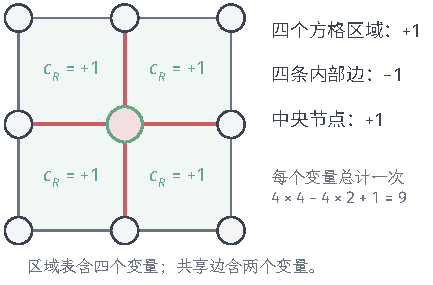
\includegraphics[width=\linewidth]{figures/03-models/03-probabilistic-graphical-models/tikz/pgm-variational-regions/figure.pdf}
  \caption{方格区域近似的计数。浅色块表示四个四变量区域，粗线标出需减去的内部边，中央节点需再加一次。每条区域一致性约束都要求大表格向交集边缘化后与小表格相同；颜色之外还用区域面积、线条和节点区分三个层次。}
  \label{fig:pgm-variational-regions}
\end{figure}

自由能怎样产生区域消息？对约束$\sum_{\bm z_{R\setminus S}}b_R-b_S=0$引入乘子$\lambda_{R,S}(\bm z_S)$。内部驻点满足
\begin{equation}
  c_R(\log b_R-\Theta_R)
    =\sum_{P:\,P\to R}\lambda_{P,R}
       -\sum_{S:\,R\to S}\lambda_{R,S}+\text{常数}.
  \label{eq:pgm-variational-region-stationarity}
\end{equation}
归一化项及$c_R$带来的常数已经合并。乘子是交集配置上的函数，因此指数化以后就是区域之间的消息。这一步同时说明为何不能把单节点消息不加修改地用于区域图：每条消息的索引现在是整个交集，且负计数区域会产生校正分母；$c_R=0$时驻点方程是乘子之间的约束，不能除以$c_R$。

在标准父子区域参数化中，还能把消息方程写成可直接计算的形式。记$\mathcal D(R)$为$R$及其全部后代，$\partial R$为所有从$\mathcal D(R)$外进入$\mathcal D(R)$的有向区域边，$\Psi_R=e^{\Theta_R}$。伪边缘写为
\[
  b_R(\bm z_R)\propto
    \Psi_R(\bm z_R)
       \prod_{(P\to Q)\in\partial R}m_{P\to Q}(\bm z_Q).
\]
这组乘子参数化将上式的计数校正纳入区域边的组合中。把它代入父子一致性并解出一条消息，得到更新方程
\begin{equation}
  m_{R\to S}(\bm z_S)\propto
  \frac{\displaystyle
    \sum_{\bm z_{R\setminus S}}
      \Psi_R(\bm z_R)
       \prod_{(P\to Q)\in\partial R}m_{P\to Q}(\bm z_Q)}
  {\displaystyle
    \Psi_S(\bm z_S)
       \prod_{\substack{(P\to Q)\in\partial S\\(P\to Q)\ne(R\to S)}}
          m_{P\to Q}(\bm z_Q)}.
  \label{eq:pgm-variational-gbp}
\end{equation}
同时出现在分子、分母且只依赖$\bm z_S$的项可先约去。消息用正值初始化，每次在父区域求和、在交集上比较并归一化，然后继续更新其他区域。这就是\term{广义置信传播}（generalized belief propagation, GBP）的一种父子消息形式。区域图须满足前述覆盖、计数和连通条件；不同冗余约束与消息规范会给出不同但相关的更新式。其固定点关系与算法构造的完整论述仍见Yedidia等人，而不是从任意重叠集合都能推出这一参数化\scite{pgm-variational-yedidia2005}

对贯穿例子，只要把三变量三角形本身选为最大区域，就需维护$8$项的表格；区域自由能退化为整个联合分布的真实自由能，最优值恰为$-\log26$。这解释了区域扩张为什么可能改进短环问题，也显示了代价。若每个变量有$k$个状态，大小为$r$的区域需要$k^r$项，交集一致性还带来额外存储与通信。一般图上不断加入区域未必单调改善Kikuchi目标或每个边缘的误差，因为熵近似也随区域选择改变。除非区域构成满足运行交集性质的精确团树等特殊情形，否则仍不能保证全局一致、自由能凸或普通GBP迭代收敛。

区域扩张同时改变伪边缘及其一致性约束；另一条路线保持成对局部多面体不变，改用树分布构造可控的熵近似。记$\rho_T>0$为生成树$T$的权重，$\sum_T\rho_T=1$，并令$\rho_{i,j}=\sum_{T:(i,j)\in T}\rho_T$为边$(i,j)$的出现率。对成对模型，正温度的\term{树重加权}（tree-reweighted, TRW）熵定义为
\begin{equation}
  \begin{aligned}
    H_{\mathrm{TRW}}(\bm b)
      &=\sum_iH(b_i)-\sum_{(i,j)\in E}\rho_{i,j}I(b_{i,j}),\\
    I(b_{i,j})
      &=\sum_{k,l}b_{i,j}(k,l)
            \log\frac{b_{i,j}(k,l)}{b_i(k)b_j(l)}.
  \end{aligned}
  \label{eq:pgm-variational-trw-entropy}
\end{equation}
这里$I$是两节点的互信息。每棵树的熵为$\sum_iH(b_i)-\sum_{(i,j)\in T}I(b_{i,j})$，所以$H_{\mathrm{TRW}}$是树熵的凸组合。对任意全局$q$，给定其树边缘的最大熵树分布的熵不小于$H(q)$；逐树加权便得$H(q)\leq H_{\mathrm{TRW}}(\bm b(q))$。因此
\begin{equation}
  A(\bm{\theta})\leq
    \max_{\bm b\in\mathcal L}
       \{\langle\bm{\theta},\bm b\rangle+H_{\mathrm{TRW}}(\bm b)\}.
  \label{eq:pgm-variational-trw-partition}
\end{equation}
树熵在树的局部一致边缘上是凹函数，可由根节点熵加沿树条件熵之和看出；其凸组合仍凹。因此这是凹目标的凸约束最大化。边出现率必须来自树分布，不能任意选正权重就宣称保有熵上界。关于配分函数上界的原始构造见Wainwright等人\scite{pgm-variational-wainwright2005partition}

Bethe在成对图中相当于把每条边的互信息都减一次；有环图上这通常不是一个生成树分布的边出现率，所以没有上述熵上界论证。TRW用于近似边缘时也不保证每个边缘比Bethe准确，上界约束的是最优目标值。它与Kikuchi分别通过树熵凸组合和更大区域修正含环图的局部自由能，不能只按区域大小排成必然改善的顺序。

\subsection{拉普拉斯近似与期望传播}
\label{sec:pgm-variational-laplace-ep}
\label{sec:pgm-variational-ep}

区域扩张主要处理依赖结构，另一些困难却来自连续后验的整体形状或单个因子的函数形式。拉普拉斯近似在一个众数附近使用整体曲率，期望传播则逐个放回难因子并匹配局部矩；两者都常产生高斯近似，却使用不同信息，也不是平均场或局部自由能路线的简单后继。

当保存完整密度会使每次更新越来越贵时，可以保留一个易计算的指数族，每次只把一个难因子暂时放回模型，计算它对重要矩的影响，再用近似族中的分布匹配这些矩。

设目标$p(\bm z)\propto p_0(\bm z)\prod_a f_a(\bm z)$，其中$p_0$容易处理，近似取$q(\bm z)\propto p_0(\bm z)\prod_a\widetilde f_a(\bm z)$。站点$\widetilde f_a$是不必单独归一化的指数族因子。\term{期望传播}（expectation propagation, EP）循环执行如下替换：
\begin{equation}
  \begin{aligned}
    q^{\setminus a}(\bm z)&\propto q(\bm z)/\widetilde f_a(\bm z),\\
    \widehat p_a(\bm z)&=
       \frac{f_a(\bm z)q^{\setminus a}(\bm z)}{Z_a},\\
    q^{\mathrm{new}}&=
       \argmin_{q'\in\mathcal Q}
           \operatorname{KL}(\widehat p_a\Vert q'),\\
    \widetilde f_a^{\mathrm{new}}(\bm z)&\propto
       q^{\mathrm{new}}(\bm z)/q^{\setminus a}(\bm z).
  \end{aligned}
  \label{eq:pgm-variational-ep}
\end{equation}
移除当前近似站点后的$q^{\setminus a}$称为\term{空腔分布}（cavity distribution），它避免同一因子被重复计算；放回真实因子得到的$\widehat p_a$称为\term{倾斜分布}（tilted distribution）。这两者必须可归一化，所匹配的矩必须存在。$Z_a$是这一步的归一化常数，不是原模型的整体配分函数。第三行作为有限KL投影，还要求倾斜分布与候选族的支持相容，至少存在一个候选使KL有限，且最小值能够在族中取得。

具体地，设$q'_{\bm{\lambda}}=h\exp\{\langle\bm{\lambda},\bm T\rangle-A_q(\bm{\lambda})\}$具有固定支持，$\widehat p_a$不在$h=0$处放置质量，$\mathbb E_{\widehat p_a}\lVert\bm T\rVert_2<\infty$。选取一个满足$\operatorname{KL}(\widehat p_a\Vert q'_{\bm{\lambda}_0})<\infty$的候选，便有
\[
  \begin{aligned}
    \operatorname{KL}(\widehat p_a\Vert q'_{\bm{\lambda}})
      ={}&\operatorname{KL}(\widehat p_a\Vert q'_{\bm{\lambda}_0})\\
       &+A_q(\bm{\lambda})-A_q(\bm{\lambda}_0)\\
       &-\langle\bm{\lambda}-\bm{\lambda}_0,
                  \mathbb E_{\widehat p_a}\bm T\rangle.
  \end{aligned}
\]
有限矩保证两个候选的对数密度比可积，因而这里没有删去无穷常数。在自然参数域内部，按式~\eqref{eq:pgm-variational-moments}对目标求导，得到
\begin{equation}
  \mathbb E_{q^{\mathrm{new}}}\bm T
     =\mathbb E_{\widehat p_a}\bm T.
  \label{eq:pgm-variational-moment-matching}
\end{equation}
在这些有限KL条件下，投影才等价于矩匹配。若目标矩在正则最小指数族的内部均值域中，严格凸性给出唯一的投影参数；若落在边界，可能只能取极限。若只知道矩存在且可实现，式~\eqref{eq:pgm-variational-moment-matching}仍可定义矩匹配更新，但不能据此称它为唯一的有限KL投影：全部候选的KL都可能为无穷大。矩不存在时，这一矩匹配更新也无法定义。对高斯族，充分统计量是$\bm z$及$\bm z\bm z^\top$，故需匹配均值和协方差。

一维例子可完整算出一次更新。令$p_0(z)=\mathcal N(z;0,1)$，只有一个因子$f(z)=\mathbb I[z\geq0]$，初始近似站点为$1$。倾斜分布是半正态分布；它与标准正态候选的KL为$\log2<\infty$，满足上述有限性条件。其归一化常数及矩为
\[
  Z_a=\frac12,\qquad
  \mathbb E_{\widehat p_a}Z=\sqrt{\frac2\pi},\qquad
  \operatorname{Var}_{\widehat p_a}(Z)=1-\frac2\pi.
\]
于是$q^{\mathrm{new}}=\mathcal N(m,v)$，$m\approx0.797885$、$v\approx0.363380$。若高斯自然参数写成$\eta z-\tau z^2/2$，新站点参数为$\tau_a=v^{-1}-1$、$\eta_a=m/v$。这一高斯仍对$z<0$分配正概率；它匹配了两个矩，却没有保留硬支持。若反过来用该高斯近似最小化$\operatorname{KL}(q\Vert p)$，KL反而无穷大。这个例子直接说明了目标方向的差异。

EP投影中的$\widehat p_a$依赖其他近似站点，故每一步并不是在最小化$\operatorname{KL}(p\Vert q)$这个全局固定目标，更不是第~\ref{sec:pgm-variational-unified}节的ELBO坐标上升。EP固定点可以与特定自由能的驻点联系起来，但普通站点迭代不保证单调或收敛。高斯站点精度可以为负，不能强求每个站点自身是概率密度；然而总体$q$、每个被使用的空腔及倾斜分布必须合法。阻尼自然参数、检查协方差正定性和监测矩残差，是实际计算所需的保护。EP的站点替换与矩匹配构造来自Minka\scite{pgm-variational-minka2001}

\label{sec:pgm-variational-laplace}

与逐因子修正的EP并行，若连续后验的主要质量集中在一个光滑峰附近，可以直接近似整个对数密度的局部形状。\term{拉普拉斯近似}（Laplace approximation）在众数附近作二阶展开，用峰的位置和曲率决定一个高斯。令$\ell(\bm z)=\log p(\bm x,\bm z)$，$\widehat{\bm z}$是内部严格局部极大点，且$\bm H=-\nabla^2\ell(\widehat{\bm z})$正定，则
\begin{equation}
  \begin{aligned}
    \ell(\bm z)&\approx\ell(\widehat{\bm z})
       -\frac12(\bm z-\widehat{\bm z})^\top
                  \bm H(\bm z-\widehat{\bm z}),\\
    q_{\mathrm L}(\bm z)&=\mathcal N(\widehat{\bm z},\bm H^{-1}),\\
    p(\bm x)&\approx
       e^{\ell(\widehat{\bm z})}(2\pi)^{d/2}|\bm H|^{-1/2}.
  \end{aligned}
  \label{eq:pgm-variational-laplace}
\end{equation}
线性项因众数处梯度为零而消失，高斯积分产生行列式项。计算上需要求众数、计算Hessian，再用Cholesky分解求解线性系统及对数行列式，不必显式求逆。如果曲率存在零方向或负方向，这个高斯尚未定义；修改Hessian以强制正定已经改变近似，不能冒称原始二阶展开。

以Gamma密度$p(z)\propto z^{a-1}e^{-bz}$、$z>0$为例，取$a>1,b>0$。众数为$\widehat z=(a-1)/b$，负二阶导数为$b^2/(a-1)$，故拉普拉斯近似为$\mathcal N((a-1)/b,(a-1)/b^2)$。当$a=3,b=1$时，它的均值、方差为$2,2$，而真实值为$3,3$，且高斯约有$7.865\%$质量落在非法的负半轴。这里的偏差来自众数不等于均值、曲率不等于整体方差，以及二阶展开没有保留支持边界。

若改用$y=\log z$，必须把Jacobian计入密度，得到$p_Y(y)\propto\exp(ay-be^y)$。在$y$坐标中，众数为$\log(a/b)$、近似方差为$1/a$；变回$z$得到对数正态近似，保证正支持，却不等于直接在$z$坐标中得到的高斯。这说明拉普拉斯近似依赖参数化，不能把坐标变换视为无关紧要的数值技巧。

二阶展开是局部陈述，整体积分近似还需要主峰支配、尾部可控等条件。若$\ell_n$随样本量$n$集中，唯一主峰附近的曲率按$n$增长，且高阶导数及尾部满足相应正则性，拉普拉斯法可形成渐近展开；仅仅存在一个正定Hessian并不推出任何有限样本误差保证。多峰时单个高斯遗漏其他峰，强偏斜或重尾时曲率也不能概括整体质量。多个峰的局部贡献可以相加，但须找到相关峰且避免错误重复计算。该方法既不天然最大化ELBO，也不给出一般的证据上界或下界\scite{bishop2006}

\subsection{结果含义、收敛与诊断}
\label{sec:pgm-variational-results-diagnostics}
\label{sec:pgm-variational-analysis}
\label{sec:pgm-variational-convergence}
\label{sec:pgm-variational-complexity}
\label{sec:pgm-variational-diagnostics}

相同的“近似后验”名称可能对应三种不同输出。平均场和结构化VI给出合法全局分布$q$，可以在$q$下计算联合事件，却受近似族限制；Bethe和Kikuchi通常只给出彼此局部一致的伪边缘，不能默认拼成全局分布；拉普拉斯近似与高斯EP给出局部高斯或指数族近似，其支持、尾部和多峰结构可能与目标不同。诊断必须先确认输出对象，再判断它能回答哪些概率查询。

同样写成消息或参数迭代，算法的逻辑保证也可能完全不同。精确平均场坐标更新使ELBO单调且有界，所以目标值收敛；若还要证明迭代点趋向驻点，需要连续性、紧的水平集、坐标子问题解的适当唯一性等条件。近似族的联合目标一般非凹，坐标最优也未必全局最优。随机变分与随机梯度允许单步下降，通常分析的是噪声受控条件下的渐近驻点，而不是每步单调。

LBP固定点存在也不等于LBP能到达它。对本章有限离散、严格正的情形，记$\psi_a$的最小、最大值为$u_a>0,v_a$，$k_i=|\mathcal X_i|$。对任意正输入，归一化后的因子到变量消息都满足$m_{a\to i}(z_i)\geq u_a/(k_iv_a)$：求和中的其他消息乘积不依赖$z_i$，用$u_a$控制分子、用$k_iv_a$控制归一化分母即可。把每条消息限制在具有这一正下界的概率单纯形内，所有消息组成的集合非空、紧且凸；将变量消息代入式~\eqref{eq:pgm-variational-lbp}后，同步更新是这个集合上的连续自映射。由Brouwer不动点定理，它至少有固定点。不能直接在允许任意零消息的单纯形边界上使用同一论证，因为多条消息的乘积可能处处为零。

这项存在性论证不包含吸引性，迭代仍可能周期振荡。存在、可达、局部稳定及自由能极小，是四个不同的性质。若因子含零，正下界消失，上述存在性证明也不再适用。EP同样只把固定点与局部矩匹配联系起来，拉普拉斯近似则依赖找到的众数和该点曲率；这些条件都不能推出边缘精度。

表~\ref{tab:pgm-variational-objectives}汇总了最容易混淆的对象。表中“无一般方向”不是说方法没有用，而是要求用边缘检查、残差或其他证据评价它，不能调用本不适用的下界定理。
\begin{table*}[htbp]
  \centering
  \begin{tabularx}{\linewidth}{l*{3}{>{\raggedright\arraybackslash}X}}
    \toprule
    方法与输出 & 优化或匹配对象 & 可用的界 & 不由此推出的结论\\
    \midrule
    平均场、结构化VI & 合法$q$的期望得分与真实熵 & ELBO不高于对数证据 & 所有边缘及尾概率都准确\\
    Bethe、Kikuchi & 局部一致表与近似熵 & 一般没有统一上下界方向 & 固定点是全局最优或真实边缘\\
    EP & 倾斜分布的局部矩匹配 & 一般没有证据界方向 & 站点更新单调提高同一ELBO\\
    拉普拉斯近似 & 众数处对数密度的二阶展开 & 一般没有证据界方向 & 峰附近曲率控制整体分布误差\\
    配分函数TRW & 树熵上界与局部多面体 & 优化值不低于对数配分函数 & 每个近似边缘都更准确\\
    MPE的LP与对偶 & 配置得分的线性松弛 & 对偶值不低于最大得分 & 分数解就是可行配置\\
    \bottomrule
  \end{tabularx}
  \caption{各方法的目标与证书。分布近似的ELBO界针对对数证据；配置近似的LP界针对最大得分。二者虽可共享局部统计量，但不能互相替代。}
  \label{tab:pgm-variational-objectives}
\end{table*}
\FloatBarrier

近似不等于计算一定便宜。设有限离散成对图有$d$个节点、$m$条边，每节点至多$k$个状态。存储一般的稠密边势需$O(mk^2)$。一次完全平均场扫描在直接计算全部边期望时通常需$O(mk^2)$，变分边缘本身只需$O(dk)$空间；Ising等特殊代数结构可以更快。一次成对LBP扫描也通常需$O(mk^2)$，但需要$O(mk)$条目保存有向消息，若显式保存边伪边缘则另需$O(mk^2)$。二者单轮量级相近，不表示迭代轮数或近似误差相近。

对于作用域$S_a$的稠密高阶因子，单次朴素局部求和本身就可能涉及$k^{|S_a|}$个配置。变分消息传递只有在充分统计量期望有简洁计算时才能绕过这个规模，不能把指数族名称当作低复杂度证明。块变分若内部树宽为$w$，表格推断通常带有$k^{w+1}$因子；Kikuchi最大区域有$r$个变量时，至少要面对$k^r$级区域表。区域方法的通信按交集状态数增长，增加区域既增加局部成本，也增加一致性校正工作。

SVI将每次全数据局部计算从$n$个样本改为$b$个样本，代价约为$bC_{\mathrm{local}}+C_{\mathrm{global}}$，其中两项分别是单样本局部更新和全局更新成本。若无需保留所有局部因子，还可避免$O(n)$份局部状态存储；总训练成本仍取决于达到目标精度所需的小批量数。摊销推断把测试时的迭代换成网络前向成本，但训练、反向传播和模型存储并没有消失。两者可以结合，分别减少每次处理的数据量和每个样本的优化量。

连续近似的瓶颈常在矩阵运算。一个$d$维稠密高斯的协方差需要$O(d^2)$空间，通用Cholesky分解需$O(d^3)$时间；拉普拉斯近似与高斯EP都可能遇到它。稀疏精度、低秩更新、分块或对角表示能改变实际代价，但也可能改变近似族。EP若每个站点作用于低维投影，可局部计算倾斜矩并利用低秩更新；不能把每次站点替换都机械地计为完整矩阵求逆。

分布近似应先问错在哪里。多峰目标可能被单峰$q$遗漏部分质量；强相关目标可能被独立近似过度压缩；硬支持与$q$不匹配时，反向KL甚至没有有限值。三角例更提醒我们，所有单节点边缘正确也不能排除联合错误。诊断应覆盖实际要用的量，例如某个变量组合的概率、预测尾部或相关系数，而不只查看单一优化曲线。

对同一固定模型，精确ELBO的提高确实意味着反向KL下降，但不保证每一个统计量的误差都逐步下降。若能获知$\varepsilon=\log p(\bm x)-\mathcal L(q)$，Pinsker不等式给出$\|q-p\|_{\mathrm{TV}}\leq\sqrt{\varepsilon/2}$；对值域在$[a,b]$内的函数$f$，有$|\mathbb E_qf-\mathbb E_pf|\leq(b-a)\sqrt{\varepsilon/2}$。困难是对数证据通常未知，单看ELBO绝对值不能获得$\varepsilon$；方差等无界统计量也不能不加矩条件使用这个界。ELBO的蒙特卡洛估计还会波动，估计值偶尔超过真实对数证据不等于理论下界失效。

可以利用重要性权重进行补充检查。若$q(\bm z)>0$覆盖$p(\bm x,\bm z)>0$的全部区域，独立采样$\bm z^{(1)},\ldots,\bm z^{(K)}\sim q$，定义
\begin{equation}
  w_k=\frac{p(\bm x,\bm z^{(k)})}{q(\bm z^{(k)})},
  \qquad
  \widehat Z_K=\frac1K\sum_{k=1}^K w_k.
  \label{eq:pgm-variational-importance}
\end{equation}
此时$\mathbb E\widehat Z_K=p(\bm x)$，而Jensen不等式给出$\mathbb E\log\widehat Z_K\leq\log p(\bm x)$，其中允许$\log0=-\infty$。这是对采样重复取期望后的界，单次$\log\widehat Z_K$不是确定性下界。仅当$\sum_kw_k>0$时，后验期望才可用$\sum_kw_kf(\bm z^{(k)})/\sum_kw_k$作自归一化估计；该比值通常存在有限样本偏差，在适当可积条件下可一致。这里要求目标被$q$覆盖，与反向KL要求$q$避开目标零区域是不同方向的支持条件。

同样仅在$\sum_kw_k>0$时，才计算基于权重的\term{有效样本量}（effective sample size, ESS）
\[
  \widehat{\mathrm{ESS}}
  =\frac{(\sum_kw_k)^2}{\sum_kw_k^2}.
\]
它衡量本批权重是否集中在少数样本上，取值介于$1$与$K$之间。$K$个样本的权重相等且为正时，ESS为$K$；只有一个权重非零时，ESS为$1$。例如实际抽了四次，权重为$(9,1,0,0)$，则ESS为$10^2/(9^2+1^2)=100/82\approx1.22$。两个样本有非零权重，但主要贡献集中于其中一个，所以ESS接近$1$，并不是在数非零权重的个数。

支持覆盖并不排除全零批次：以前面的半正态例为目标，取未归一化密度$\mathcal N(z;0,1)\mathbb I[z\geq0]$和标准正态提议，则$w_k=\mathbb I[z^{(k)}\geq0]$，全零概率为$2^{-K}$。这时$\widehat Z_K=0$仍是证据估计的一次结果，但自归一化比值和ESS均无定义，应报告“无有效加权样本”。应检查提议分布的覆盖和重叠程度，并用对数权重排查数值下溢，再考虑增加采样量；不能把全零权重改成均匀权重。

若权重极不均衡，ESS会很小，提示$q$与目标不匹配或样本数不足。但全部样本都没有到达遗漏模态时，权重可能看起来很平稳，ESS也不能发现尚未看见的质量。因此它是权重集中的诊断量，不是任意后验统计量的精度保证。若权重二阶矩不存在，常规标准误差更不可靠。多初值比较、小规模精确枚举、较丰富近似族，以及第~\ref{chap:pgm-sampling}章的采样诊断，可以提供互补证据。

另一个入口是\term{后验预测检查}（posterior predictive check）：从近似后验抽取潜变量或参数，再从观测模型生成复制数据，比较复制数据与实际数据的有意义统计量。它能揭示当前模型加推断流程未能复现的结构，却不能单独区分模型失配和推断误差。可在小问题上换成精确推断，或对同一模型比较不同推断方法，帮助定位来源；这些检查的目的不是用一条预测曲线代替所有后验校准问题\scite{pgm-murphy2012}

\section{近似MPE}
\label{sec:pgm-variational-mpe}

\subsection{从整数规划到局部多面体松弛}
\label{sec:pgm-variational-ilp-local-polytope}
\label{sec:pgm-variational-lp}

前面的输出是分布、伪边缘或局部高斯近似。现在改变查询：给定证据，要选出全部非证据变量的一组联合最优配置。本节的MPE严格沿用第~\ref{sec:pgm-elimination-mpe}节的定义，只包含纯最大化任务。一般边缘MAP含有求和变量，其目标为$\max_{\bm z_Q}\log\sum_{\bm z_R}\exp S(\bm z_Q,\bm z_R)$，明确不在本节范围内；求和与最大化的区别及正确消元顺序见第~\ref{sec:pgm-elimination-map}节。以下LP不能把$\bm z_R$也改成最大化后直接套用，否则查询已经被换成MPE。

设所有变量有限离散，证据吸收后的对数得分为
\begin{equation}
  S(\bm z)=\sum_i\theta_i(z_i)
              +\sum_a\theta_a(\bm z_{S_a}),
  \qquad M=\max_{\bm z\in D}S(\bm z).
  \label{eq:pgm-variational-mpe-score}
\end{equation}
这里的得分暂不含$-\log Z$；它不影响最优配置。先假设得分有限且至少有一个可行配置；硬约束可通过删除禁止状态或增加约束表达，不应把$-\infty$当普通LP系数输入求解器。

为把配置写成线性变量，对每个节点状态$k\in\mathcal X_i$引入$\delta_i(k)\in\{0,1\}$，对每个因子配置$\bm s\in\mathcal X_{S_a}$引入$\delta_a(\bm s)\in\{0,1\}$。要求
\begin{equation}
  \begin{aligned}
    &\sum_{k\in\mathcal X_i}\delta_i(k)=1,\qquad
       \sum_{\bm s\in\mathcal X_{S_a}}\delta_a(\bm s)=1,\\
    &\sum_{\bm s:\,s_i=k}\delta_a(\bm s)=\delta_i(k),
        \qquad i\in S_a.
  \end{aligned}
  \label{eq:pgm-variational-ilp-constraints}
\end{equation}
每个节点恰选一个标签，每个因子恰选一个与其节点标签相容的配置。最大化
\[
  \sum_{i,k}\theta_i(k)\delta_i(k)
     +\sum_{a,\bm s}\theta_a(\bm s)\delta_a(\bm s)
     =\langle\bm{\theta},\bm{\delta}\rangle
\]
就得到\term{整数线性规划}（integer linear programming, ILP）表示。给定$\bm z$可唯一构造这些指示变量；反过来，节点的唯一标签及一致性迫使每个因子也选中对应配置。这证明了整数可行解与原配置一一对应，而不只是两者目标看起来相似。

由于$\mathcal M$是全部配置指示向量的凸包，
\begin{equation}
  M=\max_{\bm{\mu}\in\mathcal M}
          \langle\bm{\theta},\bm{\mu}\rangle.
  \label{eq:pgm-variational-mpe-marginal}
\end{equation}
证明只需观察：凸组合的得分是配置得分的加权平均，不会高于最大配置得分，而最优配置本身就在凸包里。因此精确MPE也能写成连续线性优化，困难转移到了$\mathcal M$的描述，而不是凭空消失。

丢掉二值要求，只保留$\mu_i,\mu_a\geq0$及式~\eqref{eq:pgm-variational-ilp-constraints}中的线性等式，就得到局部多面体$\mathcal L$上的\term{线性规划松弛}（linear programming relaxation, LP relaxation）：
\begin{equation}
  U_{\mathrm{LP}}
     =\max_{\bm{\mu}\in\mathcal L}
               \langle\bm{\theta},\bm{\mu}\rangle,
  \qquad
  S(\widehat{\bm z})\leq M\leq U_{\mathrm{LP}}.
  \label{eq:pgm-variational-lp-bound}
\end{equation}
左侧要求$\widehat{\bm z}$是真实可行配置，右侧来自$\mathcal M\subseteq\mathcal L$。若求得的LP最优解为整数，它就是全局最优配置；若为分数，只能说得到了上界及伪边缘。LP迭代中任意一个尚未最优的原始可行分数解，其目标不一定高于$M$；实际可随时报告的上界应来自LP对偶可行解，或已获证的LP最优值。

这与第~\ref{sec:pgm-variational-laplace-ep}节的两种分布近似不同：LP保留原配置得分，放宽的是可行域，没有对数密度二阶展开，也没有倾斜矩匹配。其上界来自集合包含关系；它既不是含熵自由能的下界，也不提供后验不确定性。

三角图中，取$\mu_i(0)=\mu_i(1)=1/2$，每条边$\mu_{i,j}(0,1)=\mu_{i,j}(1,0)=1/2$，其余为$0$。这是图~\ref{fig:pgm-variational-triangle}右侧的局部一致点，得分为$3\beta$，且每条边的期望奖励至多为$\beta$，故$U_{\mathrm{LP}}=3\beta$。真实最优值只有$M=2\beta$。这个点要求三个二元变量两两不同，无法实现；其分数值不代表额外的合法配置。增加三角不等式$\sum_{(i,j)\in E}\Pr(Z_i\ne Z_j)\leq2$即可把本例的最优值压回$2\beta$，但一般图需要哪些更高阶约束，仍是计算问题。

配置优化也可看成熵消失的极限。对$\tau>0$，有限状态空间上
\[
  \max_{\bm z}S(\bm z)
  \leq \tau\log\sum_{\bm z}e^{S(\bm z)/\tau}
  \leq \max_{\bm z}S(\bm z)+\tau\log|D|.
\]
左侧取最大的一项，右侧把每一项都用最大项控制，故$\tau\downarrow0$时夹逼到$M$。由熵对偶，中间量等于$\max_{\bm{\mu}\in\mathcal M}\{\langle\bm{\theta},\bm{\mu}\rangle+\tau H^\star(\bm{\mu})\}$。这说明分布推断与配置推断为何共享几何工具，也说明两者并非同一个查询：正温度下要计入全部配置的质量，零温度下只关心最大值。

\subsection{从整体优化到对偶分解}
\label{sec:pgm-variational-dual-decomposition}
\label{sec:pgm-variational-dual-trw}

LP变量可能很多，直接交给通用求解器未必最方便。局部因子本来各自容易优化，困难是它们对共享变量必须作相同选择。\term{对偶分解}（dual decomposition）暂时允许各个子问题保有共享变量的副本，再用乘子调整各副本的得分，使它们逐渐协调。

一个能直接核验的分解将每个节点和每个因子作为子问题。对因子$a$与节点$i\in S_a$引入状态相关乘子$\lambda_{a,i}(k)$，定义
\begin{equation}
  \begin{aligned}
    D(\bm{\lambda})
       ={}&\sum_i\max_{k\in\mathcal X_i}
          \left[\theta_i(k)+\sum_{a:\,i\in S_a}\lambda_{a,i}(k)\right]\\
        &+\sum_a\max_{\bm s\in\mathcal X_{S_a}}
          \left[\theta_a(\bm s)-\sum_{i\in S_a}\lambda_{a,i}(s_i)\right].
  \end{aligned}
  \label{eq:pgm-variational-dual}
\end{equation}
对任意共同配置，把同一$z_i$代入所有副本，乘子逐项抵消，子问题得分之和等于$S(\bm z)$；各子问题独立取最大只会提高这个和。因此$D(\bm{\lambda})\geq M$对任意有限乘子成立。$D$是仿射函数的最大值之和，故凸，目标是最小化这个上界。

设节点子问题选出$k_i^\star$，因子子问题选出$\bm s_a^\star$，则
\[
  g_{a,i}(k)=\mathbb I[k_i^\star=k]-\mathbb I[s_{a,i}^\star=k]
\]
是一个次梯度，更新$\lambda_{a,i}^{(t+1)}(k)=\lambda_{a,i}^{(t)}(k)-\eta_t g_{a,i}(k)$。若节点选择了$k$而因子没有，更新降低节点对$k$的奖励，同时提高该因子对$k$的奖励，促使分歧缩小。平局时可选择任一最优配置，或在最优指示向量之间取凸组合。次梯度法单步不保证上界下降，实际应保留历次最小的$D$；也可使用有针对性的块坐标或平滑方法。

这个对偶究竟对应哪一个原问题？对局部LP的一致性等式引入同样的乘子，保留各节点、因子自己的概率单纯形约束。对每个单纯形最大化线性函数，恰好得到式~\eqref{eq:pgm-variational-dual}中的一个最大值。有限、非空且有界的LP满足强对偶，因而
\begin{equation}
  \min_{\bm{\lambda}}D(\bm{\lambda})=U_{\mathrm{LP}}\geq M.
  \label{eq:pgm-variational-dual-lp}
\end{equation}
强对偶消除的是LP与其对偶之间的间隙，不是LP与整数问题之间的间隙。若全部子问题有一个共同的最优配置，代入便同时达到$D$，于是获得精确MPE证书；若没有协调成功，则需另外构造可行配置作为下界。三角例中零乘子已经给出$D=3\beta=U_{\mathrm{LP}}$，继续优化乘子不能消除$\beta$的整数松弛间隙。

\subsection{树重加权上界}
\label{sec:pgm-variational-trw-mpe}

单因子分解以节点和因子为子问题；树分解则把多条边组合成仍可精确求解的子问题，改变上界的计算与协调方式。以下限于成对模型，且先假设原图连通；不连通时可分别处理各连通分量。令$T$遍历覆盖原图边的若干生成树，权重$\rho_T>0$满足$\sum_T\rho_T=1$。在各树上选取得分参数$\bm{\theta}^T$，树外边的参数为$0$，并要求$\bm{\theta}=\sum_T\rho_T\bm{\theta}^T$。这里分解的是得分参数，不是把后验写成普通混合分布。于是
\begin{equation}
  M\leq U_{\mathrm{TRW}}
     :=\sum_T\rho_T\max_{\bm z}
                    \langle\bm{\theta}^T,\bm T(\bm z)\rangle.
  \label{eq:pgm-variational-trw-mpe}
\end{equation}
每棵树可用最大和消息及回溯求解，乘子在树间重新分配共享项而保持加权参数和不变。\term{树重加权}（tree-reweighted, TRW）消息传递利用这种加权树分解构造和优化上界。

式~\eqref{eq:pgm-variational-trw-mpe}对任何固定参数分解都成立，但固定分解给出的$U_{\mathrm{TRW}}$可能高于$U_{\mathrm{LP}}$，因而比局部LP上界更松。若树族覆盖原图全部边，并在$\sum_T\rho_T\bm{\theta}^T=\bm{\theta}$下对所有树参数分解最小化，则树对偶施加的正是节点与边的局部一致性约束，从而
\[
  \inf_{\{\bm{\theta}^T\}}
     U_{\mathrm{TRW}}=U_{\mathrm{LP}}.
\]
因此，优化后的标准树对偶是成对局部LP的一种分解求解方式，不是必然更强的松弛。要把上界压到$U_{\mathrm{LP}}$以下，必须加入环或高阶一致性等更强约束，或引入能够施加这些约束的更大子问题；仅固定一组树或改变树权重并不能保证收紧松弛。

第~\ref{sec:pgm-variational-posterior}节的正温度TRW也能说明这一关系。把式~\eqref{eq:pgm-variational-trw-partition}中的熵乘以$\tau$并令$\tau\downarrow0$，局部集合上有界的熵项消失，得到$U_{\mathrm{LP}}$，而不必得到整数最优值$M$。零温度TRW保留的是LP松弛及其MPE上界，不再近似后验边缘。

\begin{lemma}[树一致的最优性证书]
  \label{lem:pgm-variational-tree-agreement}
  设$D$为有限非空配置集，$\mathfrak T$为有限树子问题集合，且$\rho_T>0$、$\sum_{T\in\mathfrak T}\rho_T=1$。每个树得分$S_T:D\to\mathbb R$均取有限值，并满足原问题得分分解$S(\bm z)=\sum_{T\in\mathfrak T}\rho_TS_T(\bm z)$。令
  \[
    M=\max_{\bm z\in D}S(\bm z),
    \qquad
    U_{\mathrm{TRW}}
      =\sum_{T\in\mathfrak T}\rho_T
         \max_{\bm z\in D}S_T(\bm z).
  \]
  则$U_{\mathrm{TRW}}=M$当且仅当所有树子问题具有一个共同最优配置。
\end{lemma}
\begin{proof}
  若$\bm z^\star$同时在每棵树上最优，则加权求和得到$U_{\mathrm{TRW}}=S(\bm z^\star)\leq M$，与上界合并即得等号。反之，取原问题的最优配置$\widehat{\bm z}$，则
  \[
    U_{\mathrm{TRW}}-M
      =\sum_T\rho_T
         \left[\max_{\bm z}S_T(\bm z)-S_T(\widehat{\bm z})\right].
  \]
  每个方括号非负且每个$\rho_T>0$。总和为零迫使每项为零，所以$\widehat{\bm z}$在每棵树上都最优。
\end{proof}

共同最优要求存在同一完整配置，不能仅看各节点最大边缘的候选标签集合是否相交；存在平局时，局部兼容选择还需要整体回溯。三角图有三棵生成树，各取权重$1/3$，每条边出现概率为$2/3$。将出现的边参数放大为$3\beta/2$后，加权和恢复原参数。每棵树都能使两条边不同，最优得分为$3\beta$；但三个树问题没有共同最优配置，所以其上界$3\beta$不紧。TRW的最优性证书及其与LP的关系见Wainwright等人\scite{pgm-variational-wainwright2005map}

\subsection{图割与可精确求解的特殊情形}
\label{sec:pgm-variational-graph-cut-special}
\label{sec:pgm-variational-graph-cuts}

松弛并非总会产生无法实现的最优值。有些能量结构允许直接返回整数最优配置。为说明图割，以下改用最小化能量$E(\bm z)=-S(\bm z)$；从这一处起，上界和下界的方向随符号翻转。设$z_i\in\{0,1\}$，$E(\bm z)=\sum_iD_i(z_i)+\sum_{(i,j)\in E}V_{i,j}(z_i,z_j)$，其中$D_i$和$V_{i,j}$分别为一元代价和成对代价。二元成对项满足
\begin{equation}
  V_{i,j}(0,0)+V_{i,j}(1,1)
    \leq V_{i,j}(0,1)+V_{i,j}(1,0)
  \label{eq:pgm-variational-submodular}
\end{equation}
时称为\term{次模}（submodular）。这一不等式限制的是四项的相对组合，不要求两个相同标签的能量都小于两个不同标签的能量。

\begin{theorem}[二元成对次模能量的图割表示]
  \label{thm:pgm-variational-cut}
  设$\mathcal G=(V,E)$为有限无向图，$z_i\in\{0,1\}$，且
  \[
    E(\bm z)=\sum_{i\in V}D_i(z_i)
      +\sum_{\{i,j\}\in E}V_{i,j}(z_i,z_j),
  \]
  其中所有一元项与成对项均取有限实数。若每个成对项都满足式~\eqref{eq:pgm-variational-submodular}，则能量最小化可转化为非负容量网络上的$s$--$t$最小割，最小割给出一个全局最优二元配置。
\end{theorem}
\begin{proof}
  直接应用\BookTheoremRef{thm:graph-theory-submodular-cut-representation}{第一卷“数学准备”的二值次模能量割表示定理}。
  该定理把成对项改写为一元修正与非负的$w_{i,j}|z_i-z_j|$，
  再将一元项移去共同常数，形成非负终端容量。
  本节沿用源侧取$0$、汇侧取$1$的编码，最小割配置就是MPE查询所需的合法二元答案。
\end{proof}

这一定理只讨论二元成对能量和给定标签编码。负的$w_{i,j}$不能当作合法容量；高阶因子也不由这个四项判据自动处理。图表示的更一般条件与必要性结果见Kolmogorov和Zabih\scite{pgm-variational-kolmogorov2004}

一个最小网络即可检查终端方向。取$D_1=(0,2)$、$D_2=(2,0)$、$w_{1,2}=1$，则$(0,0),(0,1),(1,0),(1,1)$的能量依次为$2,1,5,2$。图~\ref{fig:pgm-variational-cut}中最小割把节点$1$留在源侧、节点$2$放在汇侧，只支付中间容量$1$，得到最优配置$(0,1)$。这里图割不仅报告数值，还直接报告合法标签。

\begin{figure}[htbp]
  \centering
  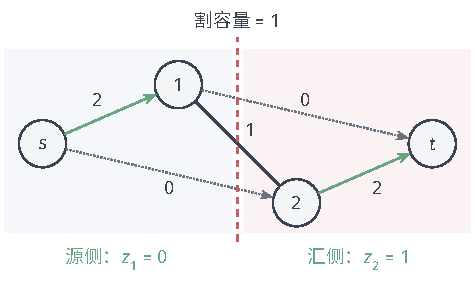
\includegraphics[width=\linewidth]{figures/03-models/03-probabilistic-graphical-models/tikz/pgm-variational-cut/figure.pdf}
  \caption{两变量次模能量的$s$--$t$割网络。实线终端边容量为$2$，点线终端边容量为$0$，中间无向边容量为$1$。虚线表示分开$\{s,1\}$和$\{2,t\}$的割，容量为$1$，对应配置$(0,1)$。}
  \label{fig:pgm-variational-cut}
\end{figure}

\subsection{紧性、取整与最优性诊断}
\label{sec:pgm-variational-tightness-rounding}

这类能量的局部LP松弛为何也紧，可以直接证明而不依赖求解器。令$m_i=\mu_i(1)$。对任何局部一致的边表，$\Pr(Z_i\ne Z_j)\geq|m_i-m_j|$，因为$m_i-m_j=\mu_{i,j}(1,0)-\mu_{i,j}(0,1)$。非负$w_{i,j}$使松弛能量不小于
\[
  C+\sum_i[(1-m_i)D'_i(0)+m_iD'_i(1)]
       +\sum_{(i,j)}w_{i,j}|m_i-m_j|.
\]
令所有节点共用$U\sim\operatorname{Uniform}(0,1)$，取$z_i=\mathbb I[U<m_i]$，则节点均值为$m_i$，不同值概率恰为$|m_i-m_j|$。这个全局分布的期望能量等于上式，所以至少有一个阈值配置的能量不高于原LP解。用于LP最优解时，结合松弛下界便得到整数最优值等于LP最优值。这证明存在整数最优解，但不保证求解器在存在平局时不会返回若干整数最优解的分数混合。按排序后的$m_i$检查至多$d+1$个阈值区间即可寻找相应配置。

树图上的局部LP也总是紧，因为局部一致表可以构造全局树分布，线性得分的期望不超过某个配置的得分。这里“紧”指最优值相等并存在整数最优解，不意味着树上每个合法边缘都是整数。含环图上的紧性则依赖结构、势函数及参数，不能仅从消息收敛判断。

对多标签变量，一次$s$--$t$割只能表达两个选项。\term{$\alpha$扩展}（$\alpha$-expansion）固定当前标签$\ell_i$，让每个节点选择保留$\ell_i$或改为$\alpha$，把这一步化为二元问题。若成对项为$w_{i,j}d(k,l)$，$w_{i,j}\geq0$且$d$是标签上的度量，三角不等式给出
\[
  d(\ell_i,\ell_j)+d(\alpha,\alpha)
    \leq d(\ell_i,\alpha)+d(\alpha,\ell_j).
\]
所以每个扩展子问题次模，能精确求解。循环标签并只接受严格改善，有限状态下会停在对所有扩展动作都无法改进的配置，但未必是全局最优。

$\alpha$--$\beta$交换只让当前标为这两个标签的节点互换，可处理某些不满足三角不等式的非负对称成对代价。对于非负一元项、非负边权的Potts能量，完全达到扩展局部最优的配置有不超过全局最优能量两倍的经典保证；这一结论依赖能量形式和停止条件，不能把它推广成任意度量、任意初次扩展或任意加常数后的能量都具有同一比值。更一般的扩展、交换与近似比结果参见Boykov等人\scite{pgm-variational-boykov2001}

有序标签和特定凸相邻代价可用多层图构造精确求解，但一般多标签或非次模能量没有这样的通用保证。某些非次模二次伪布尔松弛只能固定部分变量，其余变量还需补全；不能把“部分标签有保证”当作完整最优配置。更一般的LP分数解可以逐点选最大伪边缘、联合取整、局部搜索，或加入切平面、分支定界。逐点取整会丢失协调，硬约束存在时还可能不可行，因此必须回到原目标和原约束复核。

对得分最大化，保留已找到的最好可行值$L=S(\widehat{\bm z})$及一个经验证的对偶上界$U$，则
\begin{equation}
  0\leq M-S(\widehat{\bm z})\leq U-S(\widehat{\bm z}).
  \label{eq:pgm-variational-gap}
\end{equation}
右侧是可计算的\term{原始--对偶间隙}（primal--dual gap），在此处比较整数可行解与松弛对偶证书。若把LP原始值也记下来，还能区分求解器尚未收敛的差距和取整后的损失。对能量最小化，方向反过来：松弛或对偶提供下界，可行配置提供上界。在三角例中，逐点按平局选$0$得到得分$0$；把任一变量翻转便达到$2\beta$，但LP上界仍为$3\beta$。局部改进修复了取整损失，却没有修复松弛间隙。

对偶LP优化的全局最优性来自凸性及正确求解，而不是因为消息看上去像置信传播。即便$D$已收敛到$U_{\mathrm{LP}}$，仍可能没有共同整数配置。反过来，一旦找到可行配置并达到对偶值，就有全局证书，不必等待参数或消息达到某种唯一极限。TRW消息的具体调度也必须单独分析；具有凸的上界目标，不意味着任意形式的消息更新都单调优化该目标。

MPE分解把计算分配给子问题。成对树上的一次最大和及回溯需$O(|E_T|k^2)$；多棵树可并行，但共享乘子的协调和通信仍在。显式局部LP有约$O(dk+mk^2)$个变量，其求解时间不只由变量数决定，还受求解器、约束和容差影响。图割属于多项式时间的特殊精确子问题，一次扩展只解一个二元动作，整体还要计入标签轮数。衡量可扩展性时，应同时报告单轮计算、存储、通信和达到所需诊断标准的轮数。

MPE近似需要另一套记录：原约束是否满足、可行配置得分是多少、对偶上界是多少，以及它们的差距。三角图的结论可同时列出：完全平均场的对数配分函数下界为$3.119162$，结构化固定点的同类下界为$3.178054$，精确$\log Z_\beta=3.258097$，Bethe固定点的对数配分函数近似为$3.295837$。MPE方面，最好可行得分为$2\log2=1.386294$，LP与该树分解的上界为$3\log2=2.079442$。两个数列不能放到同一条“下界改善”曲线上比较，因为所约束的真值不同。

若原始--对偶间隙很小，就能控制当前配置距离最优得分的损失；它不说明后验是否集中在该配置附近，也不提供边缘概率。若间隙较大，则应继续优化对偶、改善取整、增加一致性约束，或接受一个明确量化的误差范围。报告连续松弛最优值而不报告合法配置，尚未完成配置推断任务。

\section{本章小结}
\label{sec:pgm-variational-summary}

把推断改写为优化，改变的是保留哪些概率关系以及接受哪种误差。对于后验分布，ELBO把近似程度连接到反向KL；平均场和结构化近似以合法全局分布换取可计算的期望与熵。共轭、随机更新和摊销映射分别降低局部代数、数据遍历与重复优化的成本，却不会修复近似族限制。

局部自由能直接维护伪边缘。树上的一致性与熵分解是精确的，推广到含环图后才出现Bethe与Kikuchi近似；更大区域能检查更多关系，也会增加表格代价。EP匹配临时放回真实因子后的矩，拉普拉斯近似匹配峰附近的曲率，二者保留的信息不同。固定点、局部匹配和目标改善，都须与真实边缘及尾部误差区分。

查询为全部非证据变量的MPE时，熵不参与目标，边缘多面体上的线性优化等价于选择最优配置。局部多面体给出最大得分上界，对偶分解与TRW提供证书，图割在二元次模等条件下直接返回整数最优解；这些结论不能越过边缘MAP中的求和运算。分布近似检查支持、相关性与预测，配置近似检查可行性、取整和原始--对偶间隙，两类诊断不能互相替代。
